%%%%%%%%%%%%%%%%%%%%%%%%%%%%%%%%%%%%%%%%%%%%%%%%%%%%%%%%%%%%%%%%%%%%%%%%%%%%%%%%
%2345678901234567890123456789012345678901234567890123456789012345678901234567890
%        1         2         3         4         5         6         7         8

\documentclass[letterpaper, 10 pt, conference]{ieeeconf}  % Comment this line out if you need a4paper

%\documentclass[a4paper, 10pt, conference]{ieeeconf}      % Use this line for a4 paper

\IEEEoverridecommandlockouts                              % This command is only needed if 
                                                          % you want to use the \thanks command

\overrideIEEEmargins                                      % Needed to meet printer requirements.

% The following packages can be found on http:\\www.ctan.org
\usepackage{graphics} % for pdf, bitmapped graphics files
%\usepackage{epsfig} % for postscript graphics files
%\usepackage{mathptmx} % assumes new font selection scheme installed
%\usepackage{times} % assumes new font selection scheme installed
\usepackage{amsmath} % assumes amsmath package installed
\usepackage{amssymb}  % assumes amsmath package installed
\usepackage{subcaption}
\usepackage{jeffe}
\usepackage{graphicx}
\usepackage{hyperref}

\title{\LARGE \bf
Periodic Trajectories of Mobile Robots}


\author{Alexandra Q. Nilles and Steven M. LaValle% <-this % stops a space
\thanks{A. Nilles and S. LaValle are with the Department of Computer Science, 
University of Illinois at Urbana-Champaign. Urbana, IL 61801, USA. 
        {\tt\small \{nilles2,lavalle\}@illinois.edu}}%
}


\begin{document}



\maketitle
\thispagestyle{empty}
\pagestyle{empty}


%%%%%%%%%%%%%%%%%%%%%%%%%%%%%%%%%%%%%%%%%%%%%%%%%%%%%%%%%%%%%%%%%%%%%%%%%%%%%%%%
\begin{abstract}

Differential drive robots, such as robotic vacuums, often have at least two motion
primitives: 1) travelling in straight lines, and 2) rotating in place upon
encountering an obstacle. 
In this paper, we analytically determine the location and stability
of periodic trajectories of such robots in regular polygons. This analysis leads
to simple, open-loop control schemes
that allow either predictable and stable "patrolling" dynamics, or ergodic
"exploratory" dynamics. The results are useful for controlling simple mobile
robots with minimal sensing and actuation, in spaces with known geometry.

\end{abstract}


%%%%%%%%%%%%%%%%%%%%%%%%%%%%%%%%%%%%%%%%%%%%%%%%%%%%%%%%%%%%%%%%%%%%%%%%%%%%%%%%
\section{INTRODUCTION}

Consider the path that a differential-drive mobile robot takes as it navigates a room.
This robot has two motion primitives that it can execute reliably: moving in a straight
line, and turning in place. It also has sensors that allow the robot to
determine whether it is in contact with an environmental boundary, and its
heading relative to that boundary.

Can we guarantee that the robot \textbf{patrols} the space on a repeatable, periodic path? Robots with
robust patrolling behavior have applications such as
monitoring environmental conditions in labs, warehouses, or greenhouses, where
a few fixed sensors may not give enough information.

% We may also ask if the robot will eventually visit every point on the boundary
% of the space. Guarantees on how the robot \textbf{covers} the space have applications
% for systems such as robotic vacuums.

One way to create these motion patterns for mobile robots is to augment the
robots with sensors such as cameras, and use algorithms such as SLAM to compute
a map of the space and estimate the robot's state. However, these robots are
expensive, require a large amount of computational and electrical power, and
their accuracy can be impacted by changing environmental conditions (such as low
light).

The approach of this paper is to treat the robot as a dynamical system, defined
by its motion primitives, independent from the specific hardware implementation.
This dynamical system is closely related to mathematical billiards
\cite{billiards}. In billiards, an agent travels in a straight line until
contacting a boundary of its environment, then bounces so that the incident
angle is always related to the outgoing angle by $\theta_{i} = -\theta_{o}$
(\textit{specular} bouncing, see Figure \ref{bounce_def}).

\begin{figure}[thpb]
  \centering
  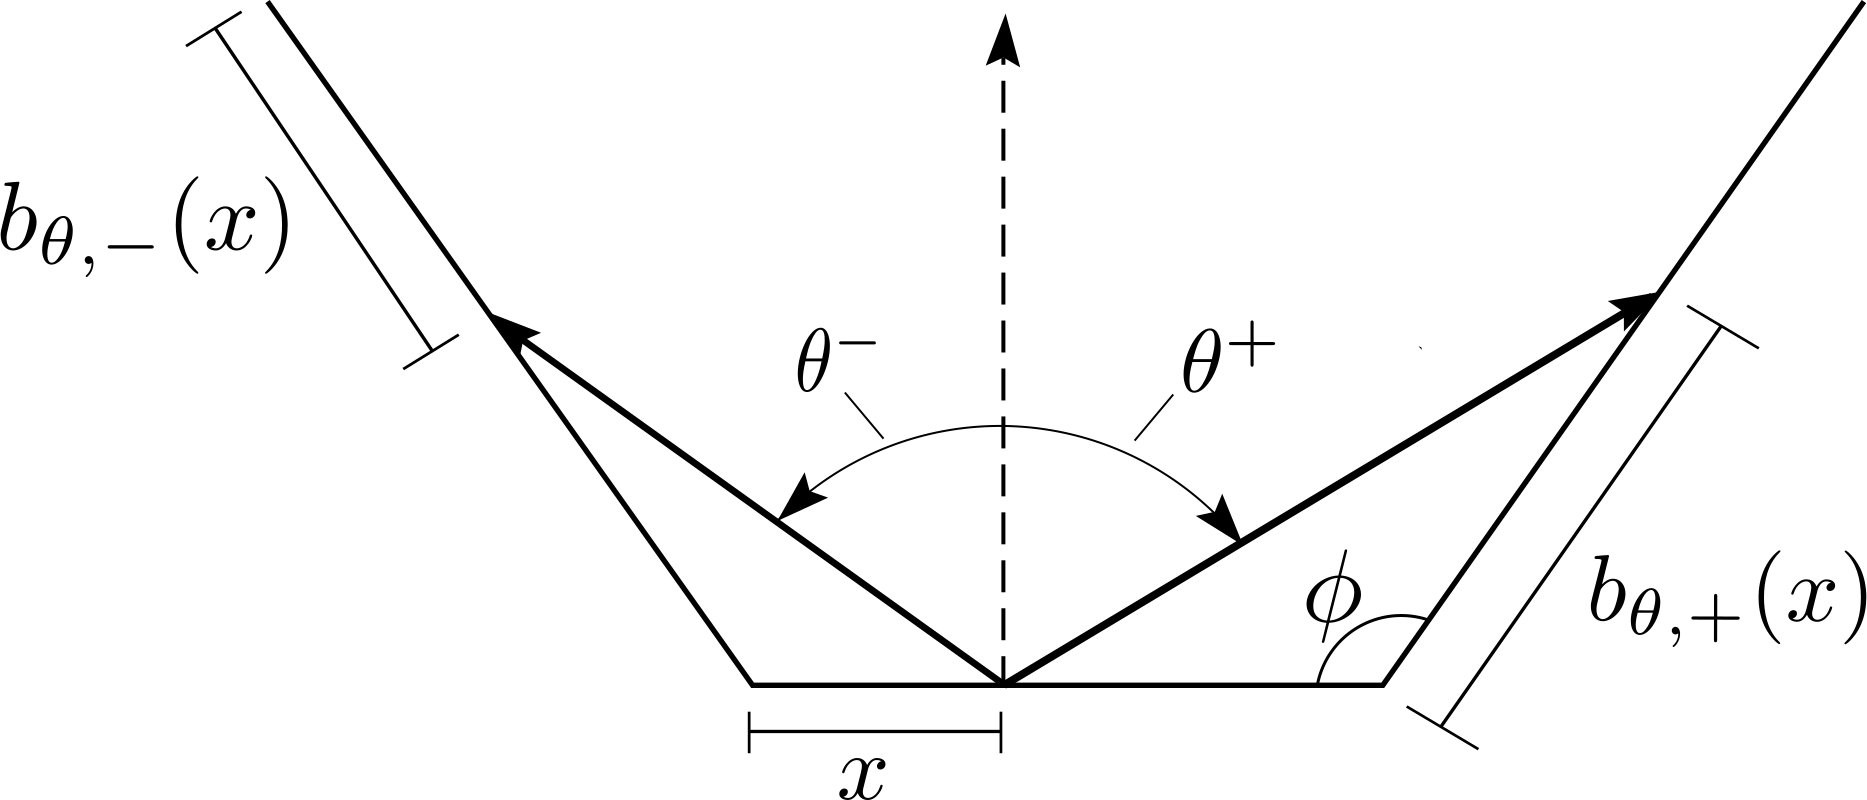
\includegraphics[width=0.3\textwidth]{figs/bounce_def.pdf}
  \caption{Definitions of the incoming angle of the
agent ($\theta_i$) and the outgoing angle ($\theta_o$), relative to the normal
vector at the point of impact.}
  \label{bounce_def}
\end{figure}

However, classical billiards is a \textit{conservative} dynamical system -
collisions are elastic, and the energy of the agent is conserved. But
robots (with energy supplies) can have nonconservative dynamics. For example, 
\textit{pinball billiards} is a model where the agent is deflected toward the
normal with each bounce, $\gamma \theta_{i} = - \theta_{o}$ for
$0 \leq \gamma \leq 1$. If the agent bounces at the normal vector
each time, this is called \textit{slap billiards}. Work in this area focuses on
analyzing the existence and structure of attractors \cite{pinball} \cite{DelMagno2014}.

The dynamical system in this paper generalizes slap billiards: the agent travels
in straight lines, and upon collision with a boundary, bounces off the boundary
at a fixed angle relative to the boundary normal vector, independent of the
incoming angle. The contributions of this paper are 1) proving the existence of
periodic orbits in $n$-sided regular polygons, and showing the range of bounce
angles that will produce periodic orbits;
2) an analysis of these orbits, showing their stability and robustness to
modeling errors; and 3) the locations where the robot collides with the polygon while
in these stable periodic orbits.

This paper is organized as follows: Section II outlines the results of the
previous paper on this model, as well as closely related work.
Section III presents the model definition and
some useful concepts from dynamical systems. Section IV analyzes the specific
case where the robot is constrained to bounce between sequential edges of the
polygon, which illustrates a technique for using the fixed point of a
trigonometric function to determine the existence and location of a periodic path.
Section V generalizes this approach to find periodic paths of period $k$ in
regular $n$-gons, when $k$ divides $n$. We then discuss possible extensions
of this work, including to more generalized polygonal environments, and
remaining open questions.


\begin{figure}

\begin{subfigure}{.25\textwidth}
\centering

\includegraphics[width=0.9\linewidth]{figs/pent_05rad.pdf}

\captionof{figure}{\sffamily\footnotesize$\theta = 1.07$ rad, 20
bounces. \label{0.5rad}}

\end{subfigure}%
\begin{subfigure}{0.25\textwidth}

\includegraphics[width=0.9\linewidth]{figs/pent_1rad.pdf}

\captionof{figure}{\sffamily\footnotesize $\theta = 0.57$ rad, 50
bounces. \label{0.57rad}}

\end{subfigure}

\begin{subfigure}{0.25\textwidth}

\includegraphics[width=0.9\linewidth]{figs/pent_165rad.pdf}

\captionof{figure}{\sffamily\footnotesize$\theta = -0.08$ rad, 75
bounces. \label{1.65rad}}

\end{subfigure}%
\begin{subfigure}{0.25\textwidth}

\includegraphics[width=0.9\linewidth]{figs/pent_3rad.pdf}

\captionof{figure}{\sffamily\footnotesize$\theta = -1.4$ rad, 20
bounces. \label{3.0rad}}

\end{subfigure}

\caption{Different behaviors of bounce trajectories in a regular pentagon.
Older bounces become 2\% more transparent with each new bounce. The circle on
the boundary indicates the starting point of the trajectory.}

\end{figure}

\section{PRIOR WORK}

Also related is work on the combinatorial complexity of the region touched
by specular bouncing ("visibility with reflection") in simple polygons
\cite{Aronov1996}. There, the authors show the combinatorial complexity of the
region touched after $k$ bounces, and provide a near-optimal algorithm for
computing the region. Our work differs by looking at non-specular bouncing and
focusing on the effects of environment symmetries on the structure of this
region.

In robotics, our model is inspired by systems such as differential drive mobile robots
with bump sensors and as few as one single-point infrared range sensors
\cite{LewOKa13}, which are able to execute the action of aligning to a specified
angle to a wall, and travelling in straight lines. This dynamical
analysis relies only on the ability to execute the two motion primitives (move
straight forward and align to $\theta$), and does not rely on any specific
hardware. \textbf{todo:} elaborate on how this shows our model is feasible

In the previous paper \cite{bounce}, the authors
characterized some of the long-term dynamics of this dynamical system. They
showed that the robot will have an orbit of period two between parallel edges,
and the robot will move monotonically ``outward" from acute vertices, or ``out" from
edges that would meet in an acute vertex if extended to their intersection.

The previous paper then defined distance- and link-unbounded
segments on arbitrary polygons, as regions of the boundary where the robot may
travel an unbounded distance while bouncing in that region or bounce an
unbounded number of times. The paper describes an algorithm for classifying the
 boundary of an arbitrary polygon into distance- and link-unbounded segments. However, the
algorithm will not terminate when the robot's trajectory converges to a periodic orbit, since in 
this case the distance- and link-unbounded regions shrink to points on the polygon
boundary, such as in Figures \ref{0.5rad} and \ref{0.57rad}.

The purpose of this paper is to begin to identify such cases -
where the dynamical system's attractor is a set of separate points, not intervals, on
$\delta P$. Then the
algorithm in \cite{bounce} can be used only for environments with attractors that are
segments on $\delta P$, for which the algorithm is guaranteed to terminate.


\section{MODEL DEFINITION}

A point robot moves in a bounded subset of the plane $P$,
defined by a continuous boundary $\delta P$, homeomorphic to  $\S^1$. For most 
of this discussion, the environment will be a simple regular polygon, so $\delta P$ 
is piecewise linear: an $n$-gon with $n$ straight edges intersecting at $n$ vertices
$(v_0, v_1, \ldots, v_{n-1})$. 

The robot drives in a straight line until encountering $\delta P$. It then rotates
until its heading is at an angle $\theta$ clockwise of the inward-facing boundary
normal, where $-\pi/2 < \theta < \pi/2$. Then the robot sets off in a
straight line again. The mapping function that these actions define between points
on $\delta P$ is $B_{\theta}: \delta P \to \delta P$, defining our dynamical system.
We will refer to this function as the \textit{bounce map}, in the same spirit as
the \textit{logistic map} in discrete dynamical systems.
When the bounce map is iterated $k$ times, we write $B^k_{\theta}$.
$B_{\theta}$ is not well defined
on vertices of $\delta P$, but the number of points where $B_{\theta}$ sends
the robot to a vertex is finite, so we will not consider such trajectories.

A sequence of points $[p_0, \ldots, p_k]$ is a \textit{flow} of $B_{\theta}$ if
$p_i = B_{\theta}(p_{i-1})$ for $1 \leq i \leq k$. A flow is an \textit{orbit} if
$B_{\theta}(p_k) = p_0$, and the \textit{period} of this orbit is $k+1$. A \textit{limit
cycle} is an orbit whose neighboring flows tend asymptotically toward or away from it
\cite{jackson1992}.


\section{BOUNCING TO SEQUENTIAL EDGES}

\textbf{Proposition 1:} In every regular $n$-sided polygon with side length $l$
and interior angle $\phi$, there exists a range for $\theta$ such that iterating
$B_{\theta}(x)$ on any $x \in \delta P$ results in a stable limit cycle of
period $n$, which strikes the boundary at points that are distance $x_{FP}$ from
the nearest clockwise vertex, with:

$$ x_{FP} = 
\begin{cases}
        \frac{l c(\theta, \phi)}{1 + c(\theta, \phi)} & \phi/2 < \theta
< \pi/2 \\
        \frac{l}{1+c(\theta, \phi)} & -\pi/2 < \theta
< -\phi/2
\end{cases}
$$

Where $c(\theta, \phi) = \cos(\theta)/\cos(\theta-\phi)$.

\textbf{Proof:} Take a regular
$n$-gon with side length $l$, and boundary $\delta P$. Let the robot begin its trajectory
at a point $p \in \delta P$ which
is at a distance $x$ from the nearest vertex in the clockwise direction.
We will begin by constraining the robot to bounce counterclockwise, at an angle
 $\theta$ such that it strikes the nearest adjacent edge, such as in Figure
\ref{0.5rad}.

Define a map $f_{\theta}: (0,l) \to (0,l)$ that takes $x$, the robot's distance from
 vertex $p_i$, and maps it to $f(x)$, the resulting distance from vertex $p_{i+
 1}$, after application of this constrained bounce map.

Then, using the triangle formed by two adjacent edges and the robot's trajectory
between them, we can solve for $f(x)$. Let $\phi=(n-2) \pi / n$ be the vertex angle of the
regular polygon.

By the law of sines:

$$ \frac{f_{\theta}(x)}{\sin (\pi/2-\theta)} = \frac{l-x}{\sin
(\pi-(\pi/2-\theta)-\phi)} $$

$$ f_{\theta}(x) = \frac{(l-x) \cos (\theta)}{\cos
(\theta-\phi)} = c (l-x) $$

By iterating this map, we find that the fixed point is:

$$ f_{\theta}^{\infty} = \sum_{i=1}^{\infty} (-l) (-c)^i = l+ \sum_{i=0}^{\infty}
(-l)(-c)^i $$

The sum is geometric, and finite when $|c| < 1$. If this condition holds, then
the fixed point becomes:

$$ f_{\theta}^{\infty} = \frac{lc}{1+c} $$

So we would expect the trajectory of a robot with bounce angle $\theta$ satisfying
$|c| < 1$ to converge to a limit cycle in the shape of an inscribed $n$-gon,
with collision points at distance $(lc)/(1+c)$ from the nearest vertex in the
clockwise direction. 

When this calculation is redone for bounces with $-pi/2 < \theta < 0$, the
resulting fixed point is $l/(1+c)$, with the same
$c=\cos(\theta)/\cos(\theta-\phi)$. Since $c \in (0,1)$ for stable orbits, we
find that the fixed point for bounces can take all values in $(0,l)$ except for
$l/2$, which would require $c=1$. \hfill $\blacksquare$

Also, note that calculating the Lyapunov exponent for the map $f_{\theta}(x)$
gives the same result: $|f_{\theta}'(x)| = c$, which implies that $|c| < 1$
gives a stable fixed point. **cite?**

This condition, $|c| < 1$, implies that a stable cycle will result for any
 $\theta$ within the bounds $\phi/2 < \theta < \pi/2$
or $-\pi/2 < \theta < -\phi/2$, which were confirmed through simulation, such as
in Figure \ref{prediction}.

\begin{figure}
\begin{subfigure}{.25\textwidth}
\centering

\includegraphics[width=0.9\linewidth]{figs/dec_limit_0pt2.pdf}

\end{subfigure}%
\begin{subfigure}{0.25\textwidth}

\includegraphics[width=0.9\linewidth]{figs/pent_limit_0pt5.pdf}

\end{subfigure}

\caption{Predicted (collisions indicated by blue dots) and simulated limit cycles when bouncing to adjacent edge in
regular polygons. \label{prediction}}
\end{figure}

\subsection{Implications for Errors in Implementations}

For each stable orbit in a given environment, we can use the bounds on
$c$ to determine the range of angles that will result in that orbit. 
Thus,
when designing a "patrolling" robot in an environment with regular polygonal
geometry, a robot designed to bounce at an angle in the center of one of these
ranges will be maximally robust to actuator or sensor errors. The resulting
maximum allowable error, $\epsilon_{max}$, will be $\pm | (\pi - \phi)/2 |$.
Bounces with error within this range will still result in stable orbits of the
workspace.

However, these orbits will impact the boundary at
a different location than expected. If there is a constant error in the bounce
angle, so that the effective bounce angle is $\theta + \epsilon$, with $\epsilon
< \epsilon_{max}$, the resulting difference in the location of the collision point
on each edge will be $\Delta_x = f_{\theta + \epsilon}^{\infty} - f_{\theta}^{\infty}$.

It is likely that physical implementations of the required motion primitives
will be imperfect - for example, differential drive robots can have assymetries
in the motors powering each wheel, which would result in a slightly curved path
through the interior of the environment, or a slight under- or over-turning
while aligning to $\theta$. These differences between the model and the
implementation may be a constant offset, $\theta + \epsilon$ - or
they may be time-varying. **todo bound error from independent random $\epsilon$
at each stage**

\section{GENERALIZATION}

\textbf{Proposition 2:} In every regular $n$-sided polygon, there exists a stable limit
cycle with period $k$ for all $k$ such that $k > 1$ and $k|n$.

\textbf{Proof:} By induction: for all prime $n$, $n \geq 3$, the statement is true by
Proposition 1, since $k=n$ and Proposition 1 guarantees a stable limit cycle that strikes
each edge sequentially.

Assume the statement is true for all $n' < n$. Then Proposition 1 guarantees a stable
limit cycle that strikes each edge of an $n$-sided polygon sequentially. For all
$k$ such that $k|n$, we can choose $k$ edges of the $n$-gon such that the edges
are equally spaced. We can then imagine extending these edges to their
intersection points, forming a regular $k$-gon. By Proposition 1, the bounce map in this
regular $k$-gon is guaranteed to induce a stable limit cycle, with collision
points at parameter $x$ on the edge for all $x$ except the very center point
of the edge. Thus $\theta$ can be chosen such that the bounce map sends the
robot to every $(n/k)-th$ edge such that the trajectory will converge to a
stable cycle with period $k$. Thus by induction, the statement is true for all
$n \geq 3$. \hfill $\blacksquare$

\textbf{Theorem 1:} In every regular $n$-sided polygon with side length $l$, if $k|n$,
there exists a stable periodic orbit with $k$ bounces where each collision with
the polygon boundary is at a distance $x$ ($0 < x < l$) from the nearest vertex in
the clockwise direction. **todo: x as function of k** 

\textbf{Proof:} Instead of bouncing between adjacent edges, we may ask what happens when the
robot bounces between edge $p_0 p_1$ and edge $p_m p_{m+1}$, "skipping" $m-1$
edges, such as in Figure \ref{0.57rad} where the robot bounces off every other
edge.

Let $m \leq \lfloor n/2 \rfloor$ (if this is not the case, reflect the polygon
across the vertical center axis, solve, and reflect back).

Extend the line segments $p_0 p_1$ and $p_m p_{m+1}$ to their point of
intersection $q$, forming the triangle $p_0 p_{m+1} q$. Let $a = \angle q
p_{m+1} p_0 = \angle q p_0 p_{m+1}$, by symmetry. Let $b = \angle p_{m+1} q
p_0$. Let $A = |q p_{m+1}| = |q p_0|$ and $B = |p_{m+1} p_0|$. See Figure
\ref{gen_bounce}. Each of the sides of the polygon has length $l$, and the robot
begins its trajectory at a point which is distance $x$ from $p_0$. We wish to
find the resulting distance from point $p_m$, $f_{\theta, m}(x)$.

\begin{figure}
\centering

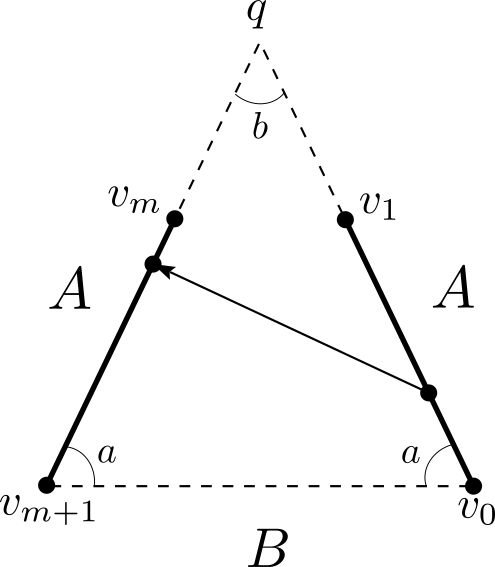
\includegraphics[width=0.2\textwidth]{figs/gen_bounce.pdf}

\captionof{figure}{A bounce from edge $p_0p_1$ to edge $p_mp_{m+1}$. The other
edges of the polygon are not drawn.
\label{gen_bounce}}

\end{figure}

Then, by the law of sines, we have:

$$ A = \frac{B \sin(a)}{\sin(b)} $$

We can then form the triangle from the points $p_0$, $p_{m+1}$, and the center
of the regular $n$-gon. The distance from the center of a regular $n$-gon to any
of its vertices is $\frac{l}{2 \sin(\pi/n)}$. The angle subtended by the edges
$p_0 p_1$ through $p_m p_{m+1}$ is $2 \pi (m+1)/n$. Thus we can solve for $B$:

$$ B = \frac{l \sin( \pi (m+1) /n)}{\sin (\pi / n)} $$

The angle $a$ can be found by considering the polygon formed by edges $p_0 p_1$
through $p_m p_{m+1}$, closed by edge $p_{m+1} p_0$. This polygon has $m+2$
vertices, so its angle sum is $m \pi$. $m$ of these vertices have the vertex
angle of the regular $n$-gon, $(n-2) \pi /n$. The remaining two vertices have
angle $a$. Therefore:

$2a + m(n-2)\pi/n = m \pi$

So $a = m \pi / n$.

And thus $A$:

$$ A = \frac{l \sin(\frac{\pi(m+1)}{n}) \sin( \frac{m \pi}{n} )}{ \sin(
\frac{\pi}{n} ) \sin( \frac{\pi(n-2m)}{n} ) } $$

Then, using the triangle formed by the the bounce of the robot, and again the
law of sines, we have:

$$ \frac{A-x}{\sin( \theta - \pi/2 + (2 \pi m)/n )} = \frac{ A - l +
f_{\theta, m}(x)}{sin(\pi/2 - \theta)} $$

Solved for $f_{\theta, m}$ and rewritten:

$$ f_{\theta, m}(x) =\frac{(x-A) \cos(\theta)}{\cos(\theta + \pi(n-2m)/n)} + l -A$$

\textbf{Observation:} When $m=1$ (agent skips no edges while bouncing around polygon), $A$
reduces to $l$, and the expression for $f_{\theta, 1}(x)$ reduces to $f_{\theta}(x)$ as 
previously derived.

\textbf{Corollary:} When $mk=n$, for some integer $k$, $A$ becomes:

\[ A = \frac{l \sin(\frac{\pi}{k} + \frac{\pi}{n}) \sin( \frac{\pi}{k} )}{ \sin(
    \frac{\pi}{n} ) \sin( \pi - \frac{2\pi}{k} } = l \left(
    \frac{\tan(\frac{\pi}{k})}{\tan(\frac{\pi}{n})} +1 \right) \]

\section{SIMULATION}

The figures and experimental simulations for this paper were computed using a
program written in Haskell and relying heavily on the excellent *Diagrams*
library \cite{diagrams}. **todo: write up on numerical precision**

The simulator is also quite general, and could be of use to those studying
classical billiards, or variants such as pinball billiards. It is also capable
of simulating random bounces, or random noise on top of a deterministic bouncing
law. Code is open source and on GitHub
\footnote{\url{https://github.com/alexandroid000/bounce}}.



\begin{table}[h]
\caption{An Example of a Table}
\label{table_example}
\begin{center}
\begin{tabular}{|c||c|}
\hline
One & Two\\
\hline
Three & Four\\
\hline
\end{tabular}
\end{center}
\end{table}



\section{DISCUSSION}

We are inspired by work on map dynamics in polygons such as
\cite{schwartz_billiards} and \cite{schwartz1992}, and it is possible that similar
techniques from projective geometry could be applied to this dynamical system.

\begin{figure}
\centering

\includegraphics[width=0.4\textwidth]{figs/squish.pdf}

\captionof{figure}{Stable limit cycles exist in polygons with fewer
symmetries than regular polygons. \label{squish}}

\end{figure}


In non-regular polygons, we cannot solve for orbits as the fixed point of one
mapping function. Yet, limit cycles still exist in polygons with enough
symmetry, as seen in Figure \ref{squish}.

\addtolength{\textheight}{-12cm}   % This command serves to balance the column lengths
                                  % on the last page of the document manually. It shortens
                                  % the textheight of the last page by a suitable amount.
                                  % This command does not take effect until the next page
                                  % so it should come on the page before the last. Make
                                  % sure that you do not shorten the textheight too much.

%%%%%%%%%%%%%%%%%%%%%%%%%%%%%%%%%%%%%%%%%%%%%%%%%%%%%%%%%%%%%%%%%%%%%%%%%%%%%%%%



%%%%%%%%%%%%%%%%%%%%%%%%%%%%%%%%%%%%%%%%%%%%%%%%%%%%%%%%%%%%%%%%%%%%%%%%%%%%%%%%



%%%%%%%%%%%%%%%%%%%%%%%%%%%%%%%%%%%%%%%%%%%%%%%%%%%%%%%%%%%%%%%%%%%%%%%%%%%%%%%%
\section*{APPENDIX}

Appendixes should appear before the acknowledgment.

\section*{ACKNOWLEDGMENT}




%%%%%%%%%%%%%%%%%%%%%%%%%%%%%%%%%%%%%%%%%%%%%%%%%%%%%%%%%%%%%%%%%%%%%%%%%%%%%%%%

\bibliographystyle{IEEEtran}
\bibliography{IEEEabrv,refs}





\end{document}
